\section{Subsystem Design}

\subsection{Preliminary Sizing}
This chapter encompasses the preliminary sizing for the aircraft. Through this process, aircraft specific values will be found, which are crucial for future engineering design decisions. For the aircraft to meet the desired aims and objectives of this project, it must be specially designed to optimise for various efficiencies along with meeting mission and performance requirements. A custom design must therefore be utilised, embodying cutting edge technologies and manufacturing methods. It also must operate purely using stored electric power, this decision was made by the authors to ensure longevity of the product moving into the future. 

\subsubsection{Theory}
For the aircraft to be successful, it must be able to carry out requirements given by its intended purpose. These requirements include both mission and performance criteria and are determined through user needs and the desired application. In order to meet these criteria and allow for further engineering in detailed design, values for weights and aerodynamic values must be estimated. Electric aircraft, in contrast to ICE-powered aircraft, do not have an existing framework for preliminary sizing. This has led to a tendency to treat most electric aircraft as prototypes, and of those that are commercially available, most are obtained through modification of existing designs. This approach is suboptimal as it leads to a lack of integration within designs, sacrificing potential efficiency gains. While some papers such as \cite{RN3} and \cite{RN85} have tried to address this issue, focusing on the sizing of a small manned electric and unmanned fixed wing eVTOL aircraft respectively, these frameworks do not fully cover the range of designs investigated within this report. Similarly, a majority of eVTOL aircraft do not have a focus on improving efficiencies in hover configurations of flight. As such, a framework that allows for optimisation in both forward and hover configurations is required. To appropriately size the aircraft, an integrated sizing method will be adopted. This will involve mixing traditional frameworks such as those described by \cite{roskam1985airplane} and \cite{raymer1989aircraft}, electric aircraft frameworks like those suggested by \cite{RN3} and \cite{RN85}, along with analysis by the authors. This will provide a more generalised framework allowing for comparison of designs and facilitation of further detailed design.

\subsubsection{Methodology}
Before the preliminary aircraft sizing can begin, statistical analysis of current systems was performed. This was used to benchmark current motors and batteries, to obtain typical specification values for specific energy, total power output, specific power, maximum power, maximum continuous power and weight. Following this and the development of the technical specifications and power requirements, the integrated approach to preliminary aircraft sizing could begin. This process is illustrated below in Figure \ref{fig:meth}.        

 
%A battery mass fraction can then be found along with PW and WS which gives us values for power, wing area, wing span and MTOW
%This data is imported into a CAD model to get values for surface area
%This is re-imported into the code and repeated until values converge. 


\begin{figure}[H]
    \centering
    \subimport{../}{PrelimSizing/method.tex}
    \caption{Preliminary Aircraft Sizing Process}
    \label{fig:meth}
\end{figure}

% \newpage
\subsubsection{Analysis}

Aircraft weights are broken down into four main categories, propulsion weight, battery weight, empty weight, and payload weight. Summing these weights as shown in Equation \ref{eq:weight} provides the total weight of the aircraft, max take off weight, denoted MTOW. 

\begin{equation}
    MTOW = W_{Prop} + W_{Batt} + W_{Empty} + W_{PL}
    \label{eq:weight}
\end{equation}

Through this analysis we will determine values for most of these weights, along with dependent aerodynamic values. $W_{PL}$ will be determined in Section \ref{payload}. $W_{Empty}$ on the other hand will be estimated as a fraction of the total weight resulting in Equation \ref{eq:weight2}

\begin{equation}
    MTOW = \dfrac{W_{Prop} + W_{Batt} + W_{PL}}{1 - MF_{empty}} 
    \label{eq:weight2}
\end{equation}

\paragraph{Statistical Analysis}
Initially current technologies were analysed in order to obtain real world expected values for COTS components. The two main components that were needed for this analysis were motors and batteries. For the motor analysis was based off of brushless electric DC motors (BLDC), these were selected due to large availability of sizes as well as favorable power to weight ratios. These motors are controlled via electronic speed controllers which again, are available in a large range of sizes. A selection of motors was cataloged with data shown in Appendix \ref{StatDATA}. These values were plotted in Figure \ref{fig:statmot}.

\begin{figure}[H]
    \centering
    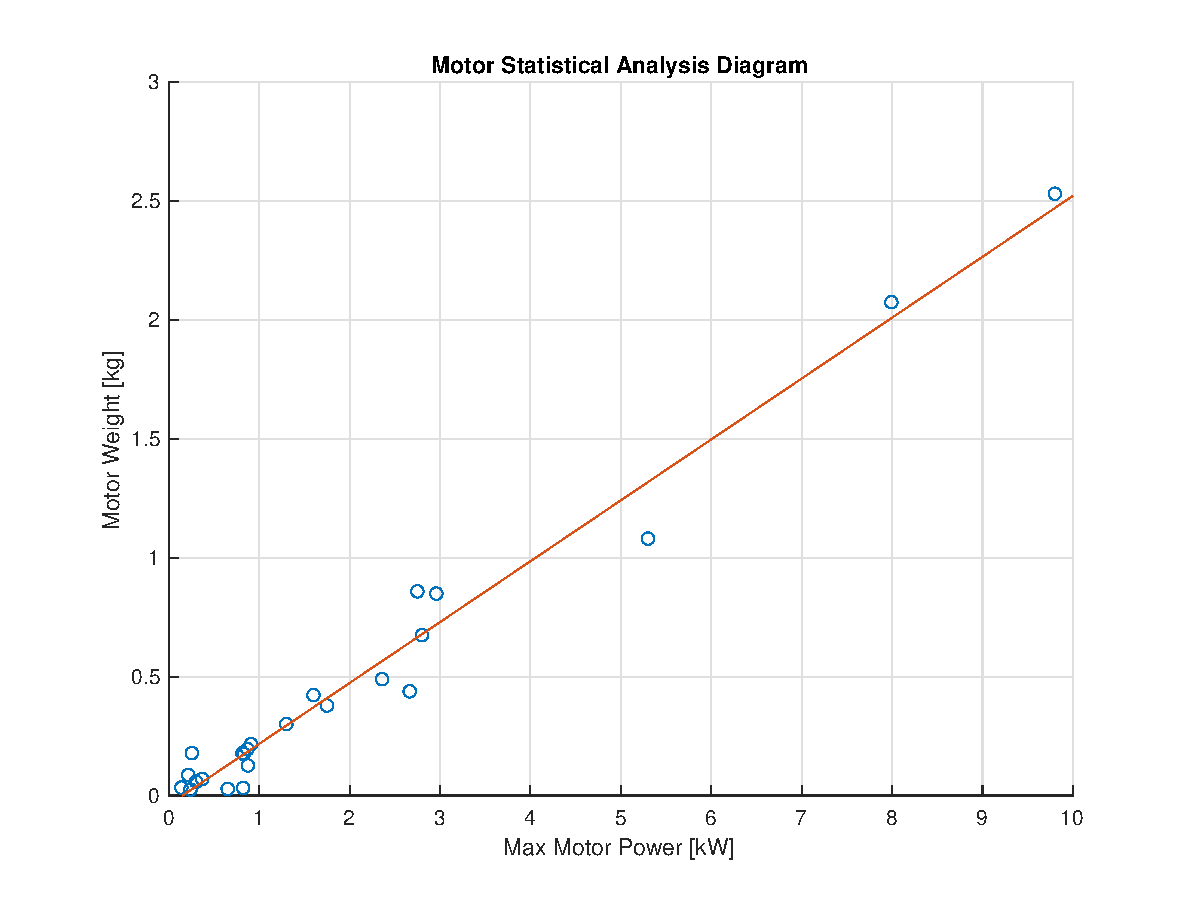
\includegraphics[width = 0.8\textwidth]{PrelimSizing/motors.eps}
    \caption{Brushless DC motor Max Power vs. Motor Weight}
    \label{fig:statmot}
\end{figure}

These values have a high degree of correlation allowing for a rough trend-line to be established, this along with the frame work detailed previously allows for an estimate of motor weight to be calculated via Equation \ref{eq:1}. 

\begin{equation}
    W_{motor} = 0.256\cdot P_{max} - 0.039
    \label{eq:1}
\end{equation}


For battery analysis, specific energy $e_{batt}$ forms the largest constraint to aircraft design. For the aircraft to complete a given mission, a fixed energy value is expended. Therefore, a battery with a greater specific energy will reduce overall weight of the drone, which in turn will reduce energy expended, increasing overall system efficiency. Another limitation of the battery is the tendency for loss of capacity over the intended life cycle. A method for prolonging battery life is to decrease the depth of discharge, however this effectively reduces the overall specific energy of the battery, therefore a battery with high specific energy and low capacity loss is preferred. For the initial sizing of this aircraft conventional lithium-ion polymer batteries (Li-po) will be selected. These have a modest specific energy of 100–265 W$\cdot$h/kg \note{CITE}{}. While this does provide some limitations, higher specific energy batteries developed in the future can be easily integrated into the existing design boosting both application and payload capabilities.  

\vspace{1cm}

Figure \ref{fig:statbatt} depicts a comparison of various COTS Li-Po batteries comparing total stored energy and battery weight. This produces a trend-line which is not linear, this can be attributed to COTS batteries including cables and a protective housing. This is more noticeable in batteries of lower weight as these auxiliary components make up less of the overall weight as total weight increases.
\begin{figure}[H]
    \centering
    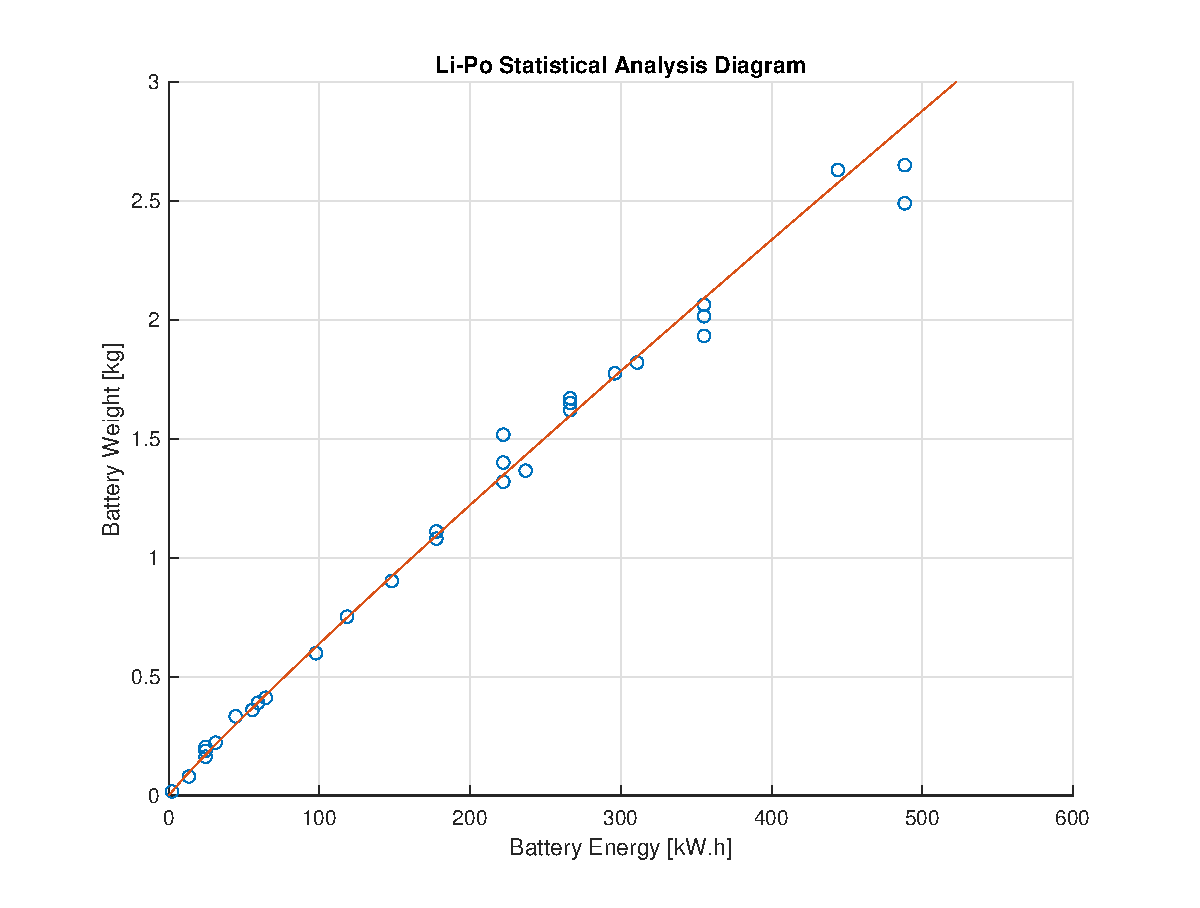
\includegraphics[width = 0.8\textwidth]{PrelimSizing/lipo.eps}
    \caption{Li-po Battery Weight vs. Total Energy}
    \label{fig:statbatt}
\end{figure}

The slope of the trend-line is equal to $1/e_{batt}$, at the higher battery weights this gives an $e_{batt}$ value of 184.45 W$\cdot$h/kg, which is comparable to literature. This analysis gives Equation \ref{eq:2}.

\begin{equation}
    W_{batt} = 0.0086\cdot E_{batt}^{0.9354}
    \label{eq:2}
\end{equation}



\paragraph{Battery Weight Analysis}

For battery weight calculations, it is defined by Equation \ref{eq:batt}. This provides a battery weight for any given specific energy and required energy. The propulsive efficiency of the system is denoted by $\eta_p$. The fraction of the battery used is represented by $F_{use}$, and determines the effective life span of the battery. More specifically, $\eta_p$ should account for efficiency losses or gains within the propulsor, motor, ESC, and current loss in connecting cables. The safety factor $SF$ considers the desired lifespan of the battery, accounting for loss of capacity. 


\begin{equation}
    W_{batt} = \dfrac{SF}{\eta_p*F_{use}} \cdot \left[ \dfrac{E_{Req}}{e_{batt}} \right]
    \label{eq:batt}
\end{equation}

If hover flight is considered, hover propulsive efficiency may be significantly different to conventional flight therefore Equation \ref{eq:batt2} is obtained.

\begin{equation}
    W_{batt} = \dfrac{SF}{F_{use}} \cdot \left[ \dfrac{\dfrac{E_{Req, FW}}{\eta_{p, FW}} + \dfrac{E_{Req, hover}}{\eta_{p, hover}}}{e_{batt}} \right]
    \label{eq:batt2}
\end{equation}

To solve this equation, values for required energy are needed for both forward and hover configurations. This was done by combining Equations \ref{eq:energy} and \ref{eq:power}.
\begin{align}
    E_{Req} &= P_{Req}\cdot t \label{eq:energy}\\
    P_{Req} &= T_{Req} \cdot v_{\infty} \label{eq:power}
\end{align}

As each flight segment has differing power requirements and duration's, mission energy requirement is given by Equation \ref{eq:missionPower}. 

\begin{equation}
    E_{Req} = \sum_{n=1}^{N} E_{Req, i}
    \label{eq:missionPower}
\end{equation}

Therefore each segments energy is given by Equation \ref{eq:segment}. 

\begin{equation}
    E_{Req, i} = \left[T_{Req, i} \cdot v_{\infty, i}\right] \cdot t_i
    \label{eq:segment}
\end{equation}

During the hover configurations of flight this equation breaks down as free-stream velocity is negligible. Therefore we must account for induced velocity produced by the propulsors. Therefore, for hover components of the mission Equation \ref{eq:hovs} is used.

\begin{equation}
    E_{Req, i, hover} = \left[T_{Req, i} \cdot \sqrt{\dfrac{T_{Req, i}}{2*A*\rho}} + v_{\infty, i}*D\right] \cdot t_i
    \label{eq:hovs}
\end{equation}



Values for segment free-stream velocity and time are given by Technical Requirement in Section 3 of this report. To find segment thrust requirements, free body analysis was conducted. It was assumed that over the span of the mission, segment transitions would be negligible, aircraft is in steady state for all mission segments, motors would idle for descent stages of flight and are not considered to have additional energy requirements. Auxiliary calculations are provided within Appendix \ref{}.


\paragraph{Empty Weight Analysis}
\note{JAKE}{Peter to write, will only be a small paragraph}


\paragraph{Constraints Analysis}
To obtain weight and power requirements found in previous sections, values for aerodynamic parameters must also be obtained. These values, such as wing area, aspect ratio, Oswald efficiency as well as lift and drag coefficients. To achieve this we need to relate weight, power and these aerodynamic parameters.\\


For conventional flight these constraints can be found using a similar process to the Roskam method \cite{roskam1985airplane} by rearranging basic lift and drag equations in terms of thrust and wing loadings. The conventional flight constraints were found for cruise, climb, stall, and flight ceiling. These are listed in Equations \ref{eq:cruise} to \ref{eq:ceiling}.
\begin{align}
    \dfrac{T}{W}_{cruise} &= q \cdot Cd_o\cdot \dfrac{S}{W}+\dfrac{k}{q}\cdot \dfrac{W}{S} \label{eq:cruise}\\
    \dfrac{T}{W}_{climb} &=  \dfrac{RC}{\cdot \sqrt{\dfrac{2}{\rho}\cdot \dfrac{W}{S}\cdot \sqrt{3\cdot Cd_o/k}}} + q \cdot Cd_o\cdot \dfrac{S}{W}+\dfrac{k}{q}\cdot \dfrac{W}{S} \label{eq:climb}\\
    \dfrac{T}{W}_{stall} &= \dfrac{1}{2}\cdot \rho \cdot v_{stall}^2 \cdot Cl_{max} \label{eq:stall}\\
    \dfrac{T}{W}_{ceiling} &= \dfrac{1}{2\cdot \sqrt{\dfrac{2}{\rho}\cdot \dfrac{W}{S}\cdot \sqrt{3\cdot Cd_o/k}}} + q \cdot \dfrac{S}{W}\cdot Cd_o + \dfrac{k}{q}\cdot \dfrac{W}{S} \label{eq:ceiling}
\end{align}

For hover, only the vertical climb segment of the flight has been considered. This is due to this segment of flight having the highest thrust and power requirements for hover configuration. This constraint is shown in Equation \ref{eq:vtolclomb}.

\begin{equation}
        \dfrac{T}{W}_{vertical climb} = SF\cdot \left(
        1 + \dfrac{1}{2}\cdot \dfrac{S}{W}\cdot V_{\infty}\cdot Cd_{V}
        \right)
    \label{eq:vtolclomb}
\end{equation}

These were then transformed to relate power loading and wing loading using Equation \ref{eq:power}. 

\begin{equation}
        \dfrac{P}{W}_{i} = \dfrac{T}{W}_{i} \cdot \dfrac{v_{\infty, i}}{\eta_{p, i}}
    \label{eq:power}
\end{equation}

From this analysis, all required information has been collected such that for a given mission, and defined technical requirements, a preliminary solution can be generated. 
\subsubsection{Results}
This analysis was mainly conducted using MATLAB, with the code found in Appendix \ref{appendixcalcs}. The results presented in this report are those of the scaled test airframe. \\

A matching diagram was generated from the constrains analysis. This diagram, depicted in Figure \ref{fig:matchingdaig}, displays the power and wing loading constraints for the aircraft. For the design to be successful it must meet all power requirements of the mission profile, this leads to a narrowing down of potential design points to those with a power loading greater then the VTOL climb constraint line. High wing loading effects an aircraft's ability to respond to gusts, its stall speed, as well reducing maneuverability. To meet mission requirements we therefore must design the aircraft with a lower wing loading then the limit imposed by its stall speed. Therefore a design area is found. From this, optimising for design requirements, A design point is selected denoted by $P_1$ on the matching diagram.

\begin{figure}[H]
    \centering
    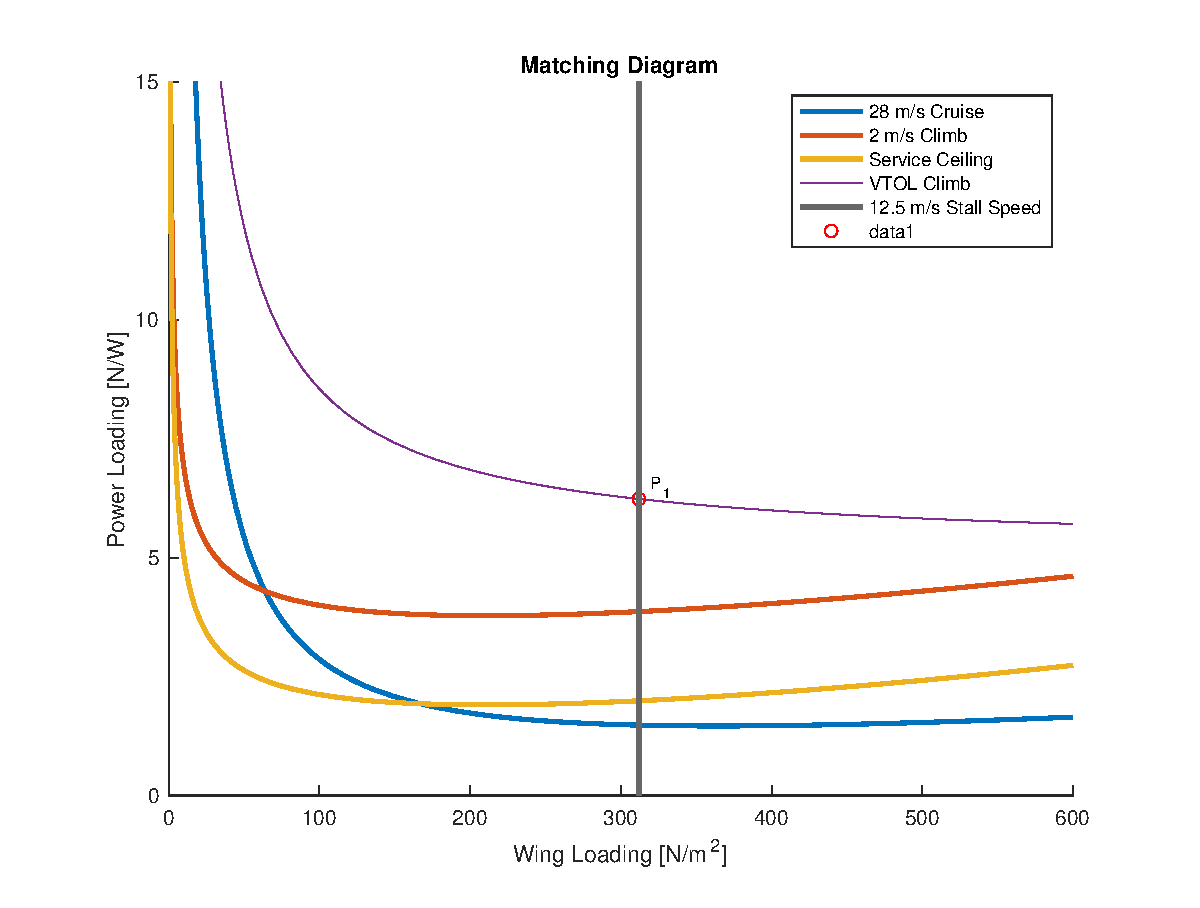
\includegraphics[width = 0.9\textwidth]{PrelimSizing/matching1.eps}
    \caption{Matching Diagram for Scaled Test Air-frame}
    \label{fig:matchingdaig}
\end{figure}

With this design point selected, analysis for the preliminary weights and aerodynamic parameters can be conducted. For convergence to occur it was found that 6 iterations were required. The preliminary values found after these 6 iterations are depicted in Table \ref{tab:preresults}.

\begin{table}[H]
\centering
\caption{Preliminary Values}
\label{tab:preresults}
\begin{tabular}{|c|c|c|}
\hline
Parameter & Value & Unit \\ \hline\hline
$M_{TOW}$ & 6.73 & $kg$ \\ \hline
$M_{Prop}$ & 0.185 & $kg$ \\ \hline
$M_{Batt}$ & 3.185 & $kg$ \\ \hline
$M_{Empty}$ & 2.36 & $kg$ \\ \hline
$M_{PL}$ & 1.00 & $kg$ \\ \hline
S & 0.6744 & $m^2$ \\ \hline
AR & 13.6 & $-$ \\ \hline
A & 0.5 & $m^2$ \\ \hline
\end{tabular}%
\end{table}

\subsubsection{Conclusion}
\note{PEter}{IDK What to put in here}



\subsubsection{Future Work}
This process is to establish preliminary values for weights and aerodynamic parameters. Moving forward with the sizing of the aircraft, it is most likely that some these values will change with detailed design. With the selection of an airframe configuration, information gained through CAD of the system such as wetted area shall be introduced into the iteration process to get more detailed estimates. From this data, aerofoils and wing geometries can be selected along with COTS batteries and motors. Stability and control considerations will also effect the final geometry of the air-frame. \\

The area of development in battery design presents great promise for the future of electric aircraft with some studies presenting novel batteries with relatively high specific energy values. A majority of these batteries are not yet commercially available, are beyond the budget of this project, or have insufficient research to justify their use. Therefore can be integrated into the design in the future as technology improves.